\chapter{Results}

%--------------------------------------------------------------------------------------------------------
% 		Success Rate
%--------------------------------------------------------------------------------------------------------
\section{Success Rate}

\subsection{Scenario 1}
\label{sec:results_success_scenario1}

The update success rate for the first scenario with one ferry and one gateway is shown in \ref{fig:result_sccess_sim1byseed_dss}.
Success rate is shown as a function of ferry memory capacity. 
Results for two separate seeds are shown since ferry movement , and hence delivery times and success rate, are random.
The spike in success rate shown for the first simulation (seed of 128) at a memory capacity of four is an artifact of this randomness.
It can be seen from this figure that success rate increases rapidly with memory capacity.
There is a leveling effect seen when memory capacity increases beyond 30.
Since there are ten source nodes each with three properties and the storage process is intelligent about keeping only the most current updates, no packets must be discarded.
%	At this point
The fact that success rate never reaches 1, or 100\%, is an artifact of the limited simulation time.
Were the simulation to run forever and ferries to visit every source node, success rate would approach 1.

\begin{figure}[htbp]
    \begin{center}
    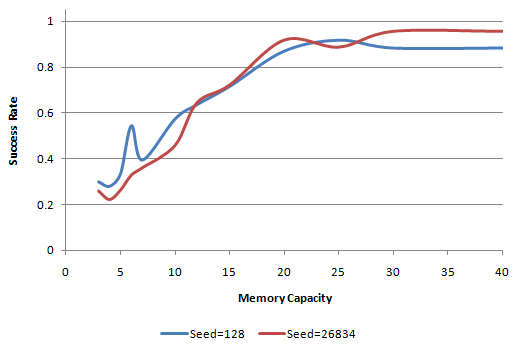
\includegraphics[width=0.8\textwidth]{images/result_sccess_sim1byseed_dss}
    \caption{Success Rate vs Memory Capacity - Simulation 1 (1 Ferry, 1 Gateway), Source Storage Disabled}
    \label{fig:result_sccess_sim1byseed_dss}
    \end{center}
\end{figure}

\subsection{Scenario 2}

The update success rate for second scenario with two ferries and two gateways is shown in \ref{fig:result_sccess_sim2byseed_dss}.
As in section \ref{sec:results_success_scenario1}, success rate is shown as a function of ferry memory capacity and results for two separate seeds are shown.
It can be seen that variability in the success rate between the two seed values is lower than the first scenario.
Increasing the number of ferries and gateways increases the likely hood a ferry will pass by the node.
%Something about gussians and decreasing variance.

\begin{figure}[htbp]
    \centering
    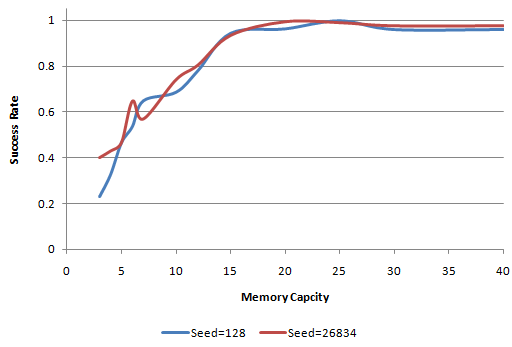
\includegraphics[width=0.8\textwidth]{images/result_sccess_sim2byseed_dss}
    \caption{Success Rate vs Memory Capacity - Simulation 2 (2 Ferries, 2 Gateways), Source Storage Disabled}
    \label{fig:result_sccess_sim2byseed_dss}
\end{figure}

\subsection{Comparison of Success Rate}

A comparison of success rate between simulations 1 and 2 is show in figure \ref{fig:result_sccess_bothsim_128_dss}.
It can be seen the additional ferry and gateway significantly increase success rate; this result is expected.
As discussed in section \ref{sec:results_success_scenario1}, the success rate should be 1 for memory capacities beyond 30. 
The fact that it is not is a result of limited simulation time.

\begin{figure}[htbp]
    \centering
    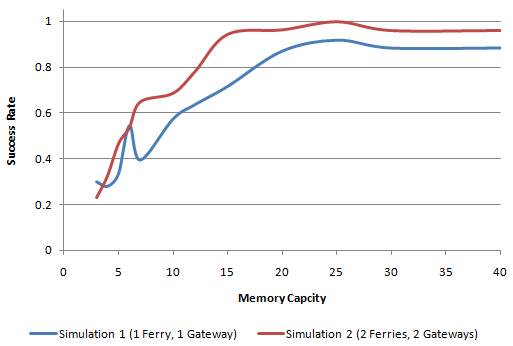
\includegraphics[width=0.8\textwidth]{images/result_sccess_bothsim_128_dss}
    \caption{Success Rate vs Memory Capacity - Simulation 1 and 2 , Seed of 128 and Source Storage Disabled}
    \label{fig:result_sccess_bothsim_128_dss}
\end{figure}

\subsection{Effect of Source Node Storage}

As discussed in section \ref{sec:source_node_storage}
\begin{figure}[htbp]
    \centering
    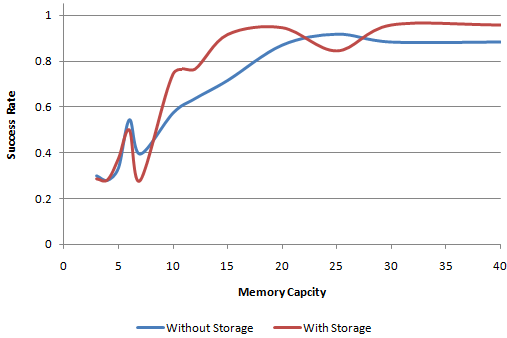
\includegraphics[width=0.8\textwidth]{images/result_sccess_sim1byss_128}
    \caption{Success Rate vs Memory Capacity - Simulation 1 and 2 , Seed of 128 and Source Storage Disabled}
    %\label{fig:result_sccess_sim1byss_128}
\end{figure}

\begin{figure}[htbp]
    \centering
    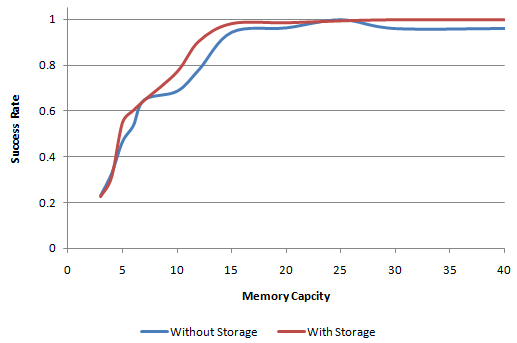
\includegraphics[width=0.8\textwidth]{images/result_sccess_sim2byss_128}
    \caption{TODO}
    %\label{fig:moistureSensor}
\end{figure}


%--------------------------------------------------------------------------------------------------------
% 		Delay
%--------------------------------------------------------------------------------------------------------
\section{Delay}

\subsection{Scenario 1}

\begin{figure}[htbp]
    \centering
    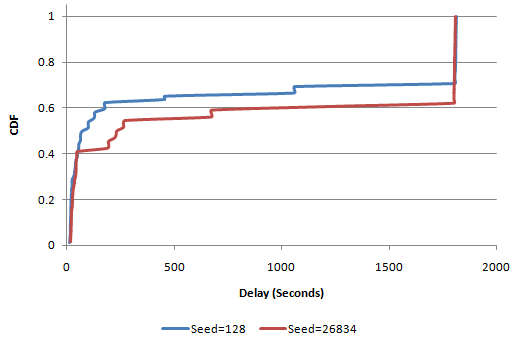
\includegraphics[width=0.8\textwidth]{images/result_delay_sim1byseed_mc3}
    \caption{TODO}
    %\label{fig:moistureSensor}
\end{figure}


\begin{figure}[htbp]
    \centering
    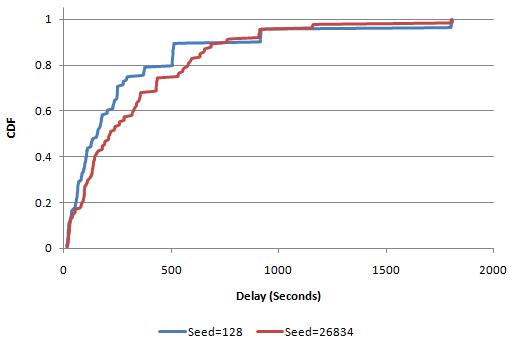
\includegraphics[width=0.8\textwidth]{images/result_delay_sim1byseed_mc30}
    \caption{TODO}
    %\label{fig:moistureSensor}
\end{figure}

\subsection{Scenario 2}

\begin{figure}[htbp]
    \centering
    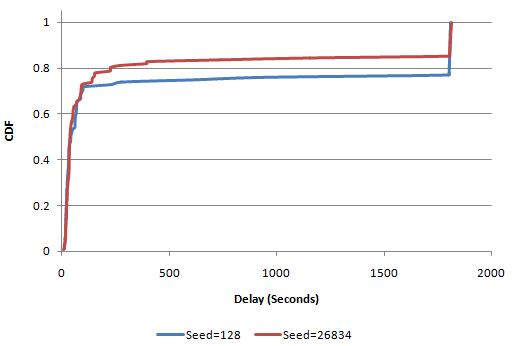
\includegraphics[width=0.8\textwidth]{images/result_delay_sim2byseed_mc3}
    \caption{TODO}
    %\label{fig:moistureSensor}
\end{figure}


\begin{figure}[htbp]
    \centering
    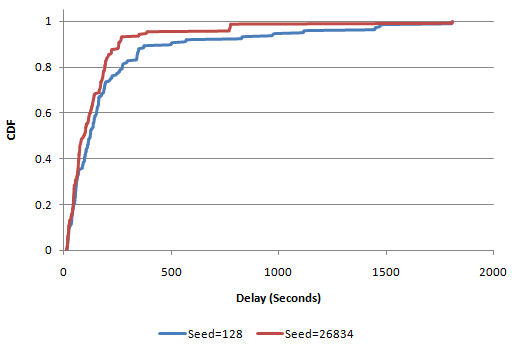
\includegraphics[width=0.8\textwidth]{images/result_delay_sim2byseed_mc30}
    \caption{TODO}
    %\label{fig:moistureSensor}
\end{figure}


\subsection{Comparison}

\begin{figure}[htbp]
    \centering
    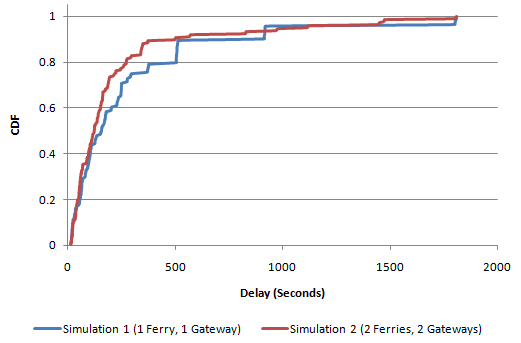
\includegraphics[width=0.8\textwidth]{images/result_delay_both_128_mc30}
    \caption{TODO}
    %\label{fig:moistureSensor}
\end{figure}


\begin{figure}[htbp]
    \centering
    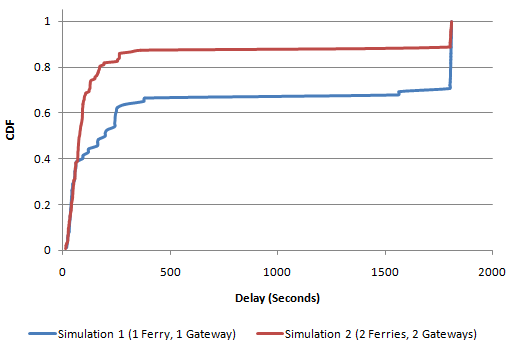
\includegraphics[width=0.8\textwidth]{images/result_delay_both_128_mc5}
    \caption{TODO}
    %\label{fig:moistureSensor}
\end{figure}